%!TEX TS-program = xelatex
\documentclass[]{friggeri-cv}
\addbibresource{bibliography.bib}

\begin{document}
\header{Wei }{Sun}
       {Game Developer}
% In the aside, each new line forces a line break
\begin{aside}
  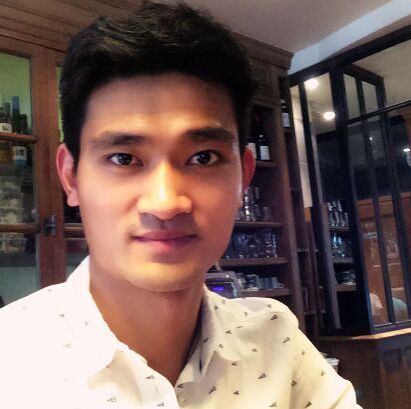
\includegraphics[width=100pt]{sunwei}
  \section{Contact}
    1068 Xueyuan Avenue
    Shenzhen University Town
    Shenzhen, China
    ~
    +86 186-8230-2496
    \href{mailto:sunwayliving@gmail.com}{sunwayliving@gmail.com}
    \href{https://github.com/sunwaylive}{\small{https://github.com/sunwaylive}}
    \href{http://www.linkedin.com/pub/sun-wei/87/626/128}{\small{www.linkedin.com/in/sunwaylive}}
  \section{Languages}
    Chinese (native)
    English (proficient)
  \section{Programming}
    {\color{red} $\varheartsuit$} C++ (proficient)
    C\# (prior experience)
    Lua (prior experience)
    Unity3D \& Unreal
\end{aside}

%----------------------------------------------------------------------------------------
%	EDUCATION SECTION
%----------------------------------------------------------------------------------------
\section{Education}
%\vspace{.1cm}
\begin{entrylist}
%------------------------------------------------
\entry
{2012 - 2015}
{Master {\normalfont in Computer Science}}
{SIAT, Chinese Academy of Sciences, China}
{Specialization in Computer Graphics and Visualization}
%------------------------------------------------
\entry
{2008 - 2012}
{Bachelor {\normalfont in Computer Science}}
{Sichuan University, China}
{\\Specialization in software engineering. 
 \\GPA: 3.57/4 (Top 2\%), CET4: 612, CET6: 513}
%------------------------------------------------
\end{entrylist}

%----------------------------------------------------------------------------------------
%	WORK EXPERIENCE SECTION
%----------------------------------------------------------------------------------------
\section{Experience}
\begin{entrylist}
     %------------------------------------------------
    \entry
    {07/2015 - Now}
    {Tencent Game Developer (C\# \& Unity3D \& C++ \& Linux )}
    {Tencent Inc}
    {\emph{} %{\emph{Siggraph Asia Project}
    \\ Write game client codes using Unity3D in Naruto mobile game team, and write game server C++ codes on Linux.
    Write rope simulation codes for ninja skill effects, and integrate game physics engine(Physx 3.3) to server. }
    %------------------------------------------------
    
    %------------------------------------------------
    \entry
    {10/2013 - 02/2014}
    {Quality Driven Poisson Guided Autoscanning ( C++ )}
    {Siggraph Asia}
    {\emph{} %{\emph{Siggraph Asia Project}
    Our algorithm is designed to instruct the PR2 robot to scan the object automaticly. I Coded our algorithm in C++, and three other state-of-art algorithms for comparisons. The thesis is submitted to Siggraph Asia 2014(international top conference in graphics). To watch the video, \href{http://v.youku.com/v_show/id_XNzQ0NTY0Mzk2.html}{\underline{please click me}}.}
    %------------------------------------------------
    %------------------------------------------------
    \entry
    {07/2013 - 09/2013}
    {CGAL - Google Summer of Code 2013 ( C++)}
    {Google, Mountain View}
    {\emph{} %{\emph{Contribution to OpenSource} 
    \\ I accelerated three algorithms in CGAL(Computer Geometry Algorithm Library) using Thread Building Block, and made them 2$\sim$6 times faster under quad core processor computer, and they have been released in CGAL version 4.4 .}
    %------------------------------------------------
    %------------------------------------------------
    \entry
    {12/2009 - 05/2010}
    {Skios Input Method ( C\# )}
    {Microsoft, Beijing}
    {\emph{} %{\emph{Imagine Cup 2010}
    \\Skios Input Method runs on windows phones. In this project, I designed words storing and searching algorithm using table-driven pattern. }
    %------------------------------------------------
    %------------------------------------------------
    \entry
    {12/2009 - 05/2010}
    {Smart Campus ( Java )}
    {Intel Corporation, Beijing}
    {\emph{} %{\emph{National Software Innovation Contest} 
    \\The system is a web application based on Zigbee-Based Internet of Things, and in the project I developed approximate half part of the functional codes, including resource status monitoring, fire alarm and so on.}
    %------------------------------------------------
\end{entrylist}

%----------------------------------------------------------------------------------------
%	Reward SECTION
%----------------------------------------------------------------------------------------
\section{Reward}
\begin{entrylist}
    %------------------------------------------------
    \entry
    {2015 - 2015}
    {Outstanding Graduate}
    {SIAT}
    {}
    
    %------------------------------------------------
    \entry
    {2014 - 2015}
    {The National Scholarship (Master Top 1\% )}
    {The Ministry of National Education}
    {}
    
    %------------------------------------------------
    \entry
    {2010 - 2011}
    {The National Scholarship (Bachelor Top 1\% )}
    {The Ministry of National Education}
    {}
    
    %------------------------------------------------
    \entry
    {2010 - 2011}
    {Double Top Ten Student (200 / 60000)}
    {Sichuan University}
    {}
    %\\Awarded to the top student both in academy performance, approximate 200 out of 60000 students including undergraduates, masters and doctors.

    %------------------------------------------------
    \entry
    {2010 - 2011}
    {Software Innovation Contest - National Second Prize}
    {Intel Corporation}
    {}

    %------------------------------------------------
    \entry
    {2009 - 2010}
    {The National Scholarship (Bachelor Top 1\% )}
    {The Ministry of National Education}
    {}
    
    %------------------------------------------------
    \entry
    {2009 - 2010}
    {Imagine Cup National Third Prize}
    {Microsoft Corporation}
    {}

\end{entrylist}

%----------------------------------------------------------------------------------------
%	Personal Character
%----------------------------------------------------------------------------------------
\section{Personal Character}
\vspace{.1cm}

\begin{entrylist}
    %------------------------------------------------
    \entry
    {Perseverance}
    {Ride a bike to Lhasa}
    {Pass Through Tibetan Autonomous Region}
    {\\In the summer of 2013, rode a bicycle to Tibet, from Xinjiang province to Tibet, 2500km, 400km depopulated district, 33 days, great experience.}
    %------------------------------------------------
    \entry
    {Leadership}
    {Chairman of Student Union}
    {SIAT, CAS}
    {\\Act as Chairman of Student Union from 2013  to 2015.}
    %------------------------------------------------
\end{entrylist}

\section{Publications}

\textbf{[1]} Wu Shihao, Sun Wei, Long Pinxin, Huang Hui, Cohen-Or Daniel, Gong Minglun, Deussen Oliver, Chen Baoquan, \textbf{Quality-driven Poisson-guided Autoscanning}, \textbf{SIGGRAPH ASIA 2014}.
		
\textbf{[2]} Kai Xu, Hui Huang, Yifei Shi, Hao Li, Pinxin Long, Jianong Caichen, Wei Sun, Baoquan Chen , \textbf{Autoscanning for Coupled Scene Reconstruction and Proactive Object Analysis}, \textbf{SIGGRAPH ASIA 2015}.

%%% This piece of code has been commented by Karol Kozioł due to biblatex errors. 
% 
%\printbibsection{article}{article in peer-reviewed journal}
%\begin{refsection}
%  \nocite{*}
%  \printbibliography[sorting=chronological, type=inproceedings, title={international peer-reviewed conferences/proceedings}, notkeyword={france}, heading=subbibliography]
%\end{refsection}
%\begin{refsection}
%  \nocite{*}
%  \printbibliography[sorting=chronological, type=inproceedings, title={local peer-reviewed conferences/proceedings}, keyword={france}, heading=subbibliography]
%\end{refsection}
%\printbibsection{misc}{other publications}
%\printbibsection{report}{research reports}

\end{document}
